\subsection{1-D test case}
\begin{frame}
\frametitle{Fixed source}
Comparison between $SP_3$ and Diffusion solutions of the scalar flux.

\begin{columns}

    \column[t]{5cm}
	\begin{figure}[htbp!]
		\begin{center}
			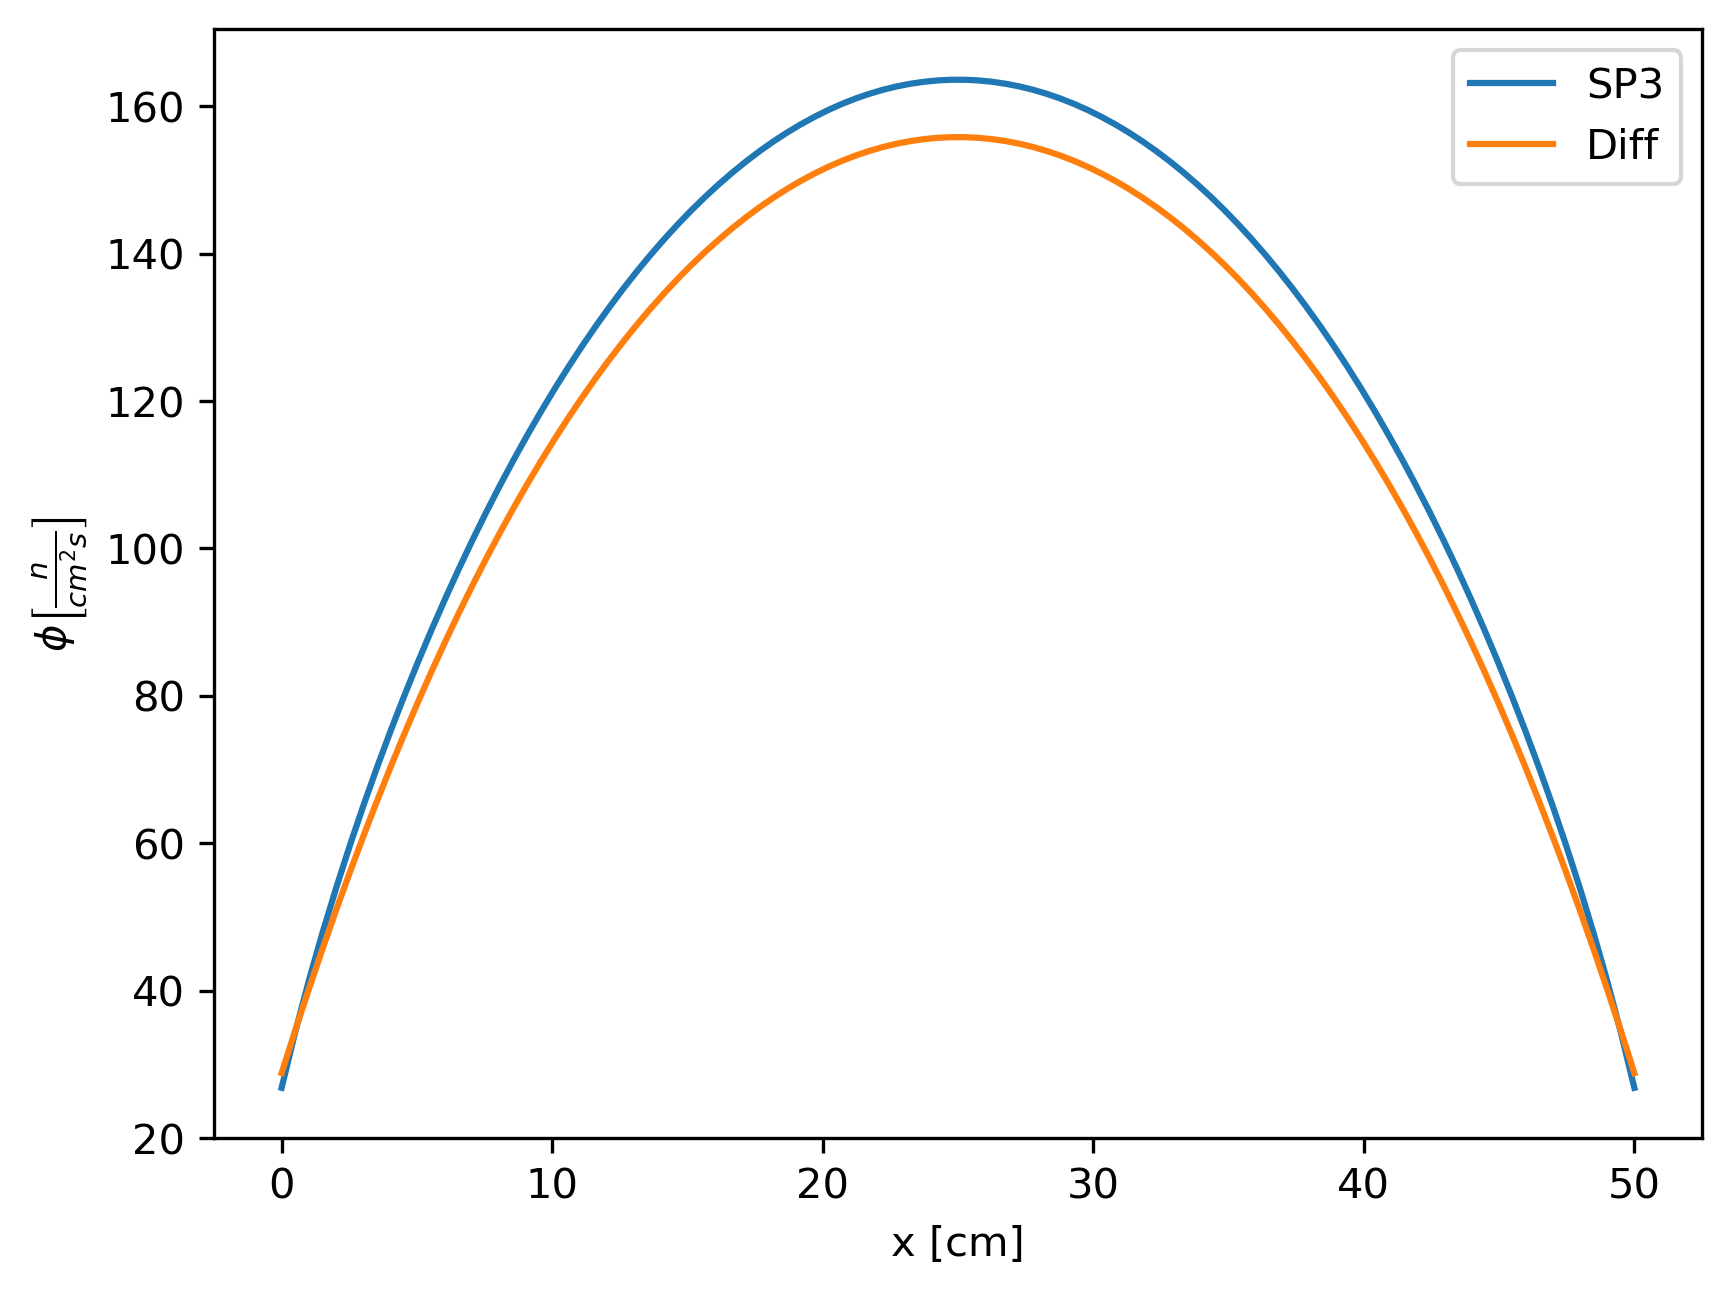
\includegraphics[height=4cm]{../sp3-diffusion/output-1g-fixed}
		\end{center}
		\caption{1 group.}
	\end{figure}

	\column[t]{5cm}
	\begin{figure}[htbp!]
		\begin{center}
			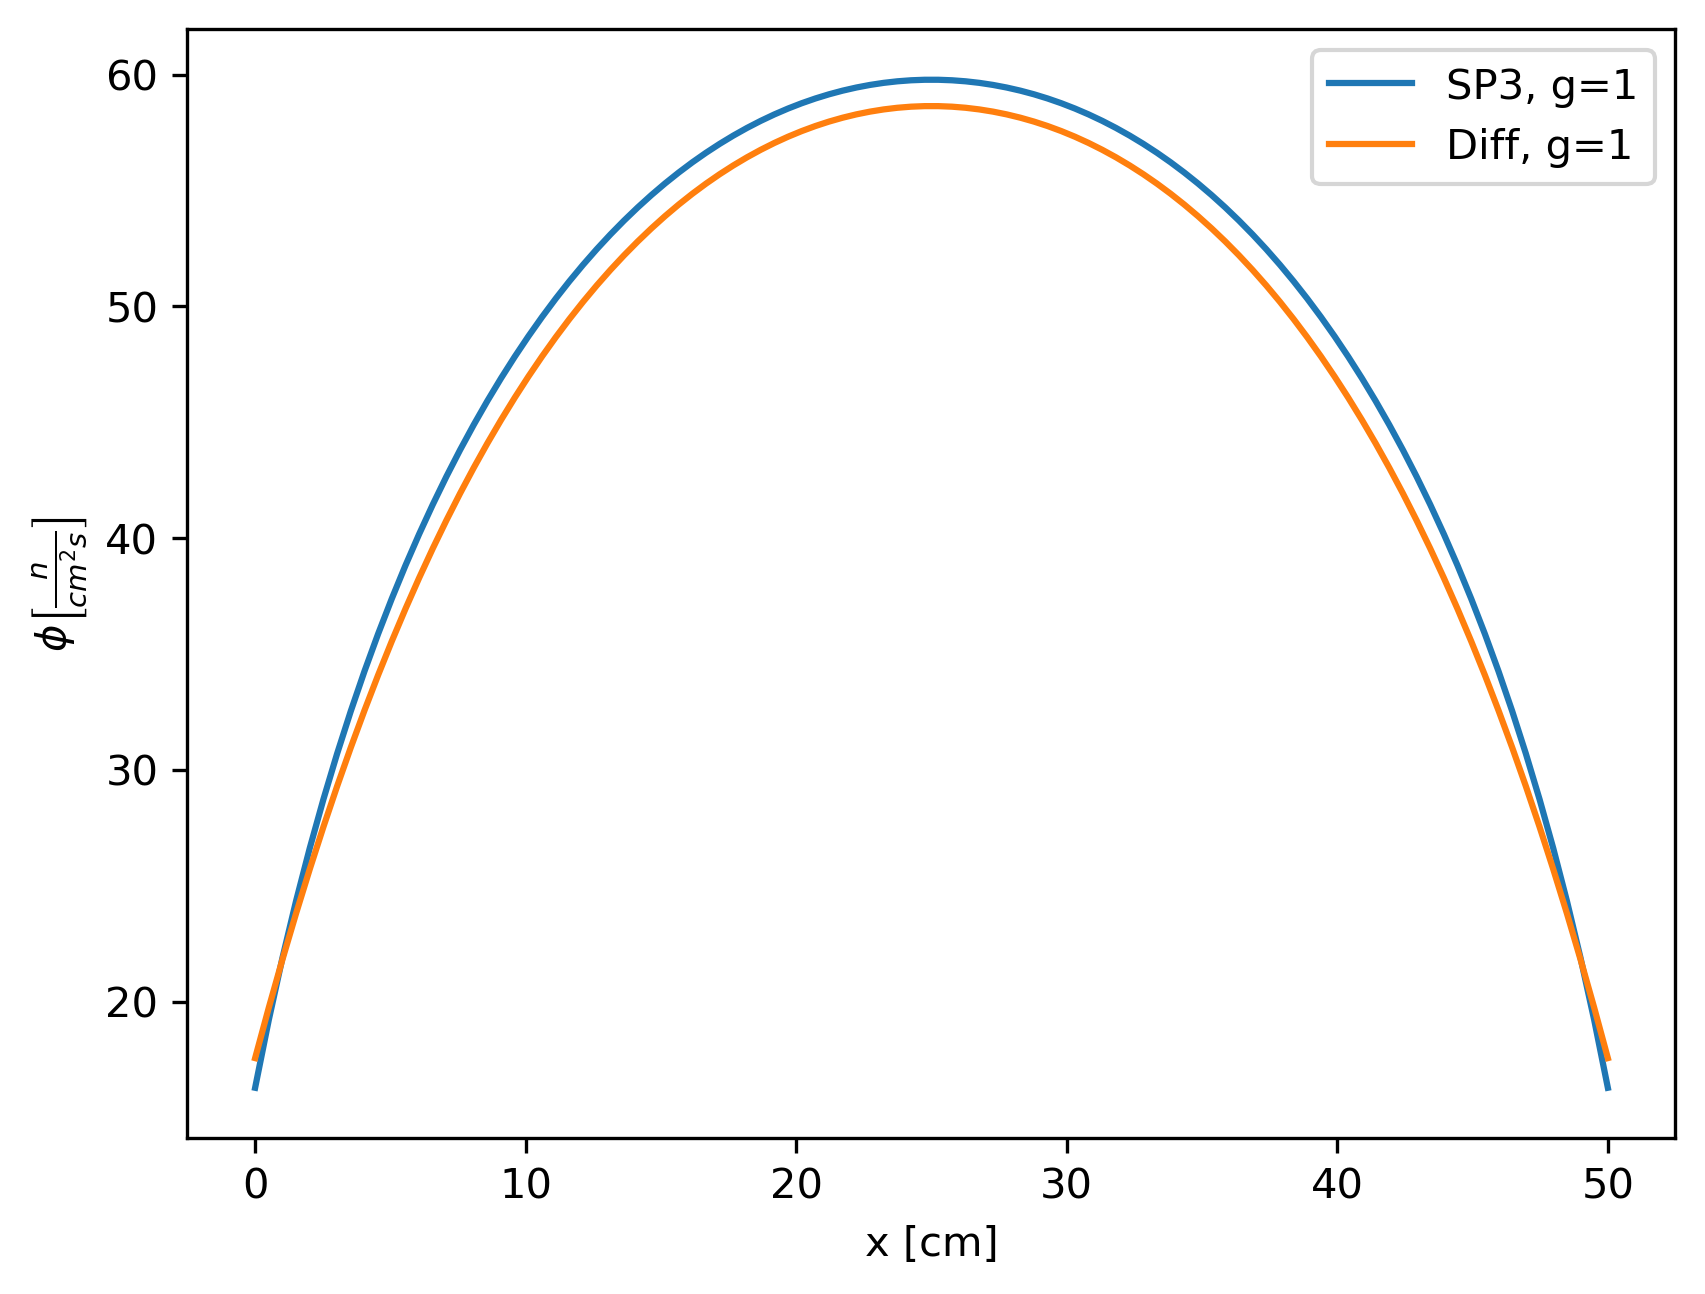
\includegraphics[height=4cm]{../sp3-diffusion/output-3g-fixed}
		\end{center}
		\caption{3 groups.}
	\end{figure}
\end{columns}
\end{frame}


\begin{frame}
\frametitle{Eigenvalue problem}

Comparison between $SP_3$ and Diffusion solutions of the scalar flux.
Solutions are normalized to the maximum value of the flux (fast flux for the 3 group case).

\begin{columns}
    \column[t]{5cm}
	\begin{figure}[htbp!]
		\begin{center}
			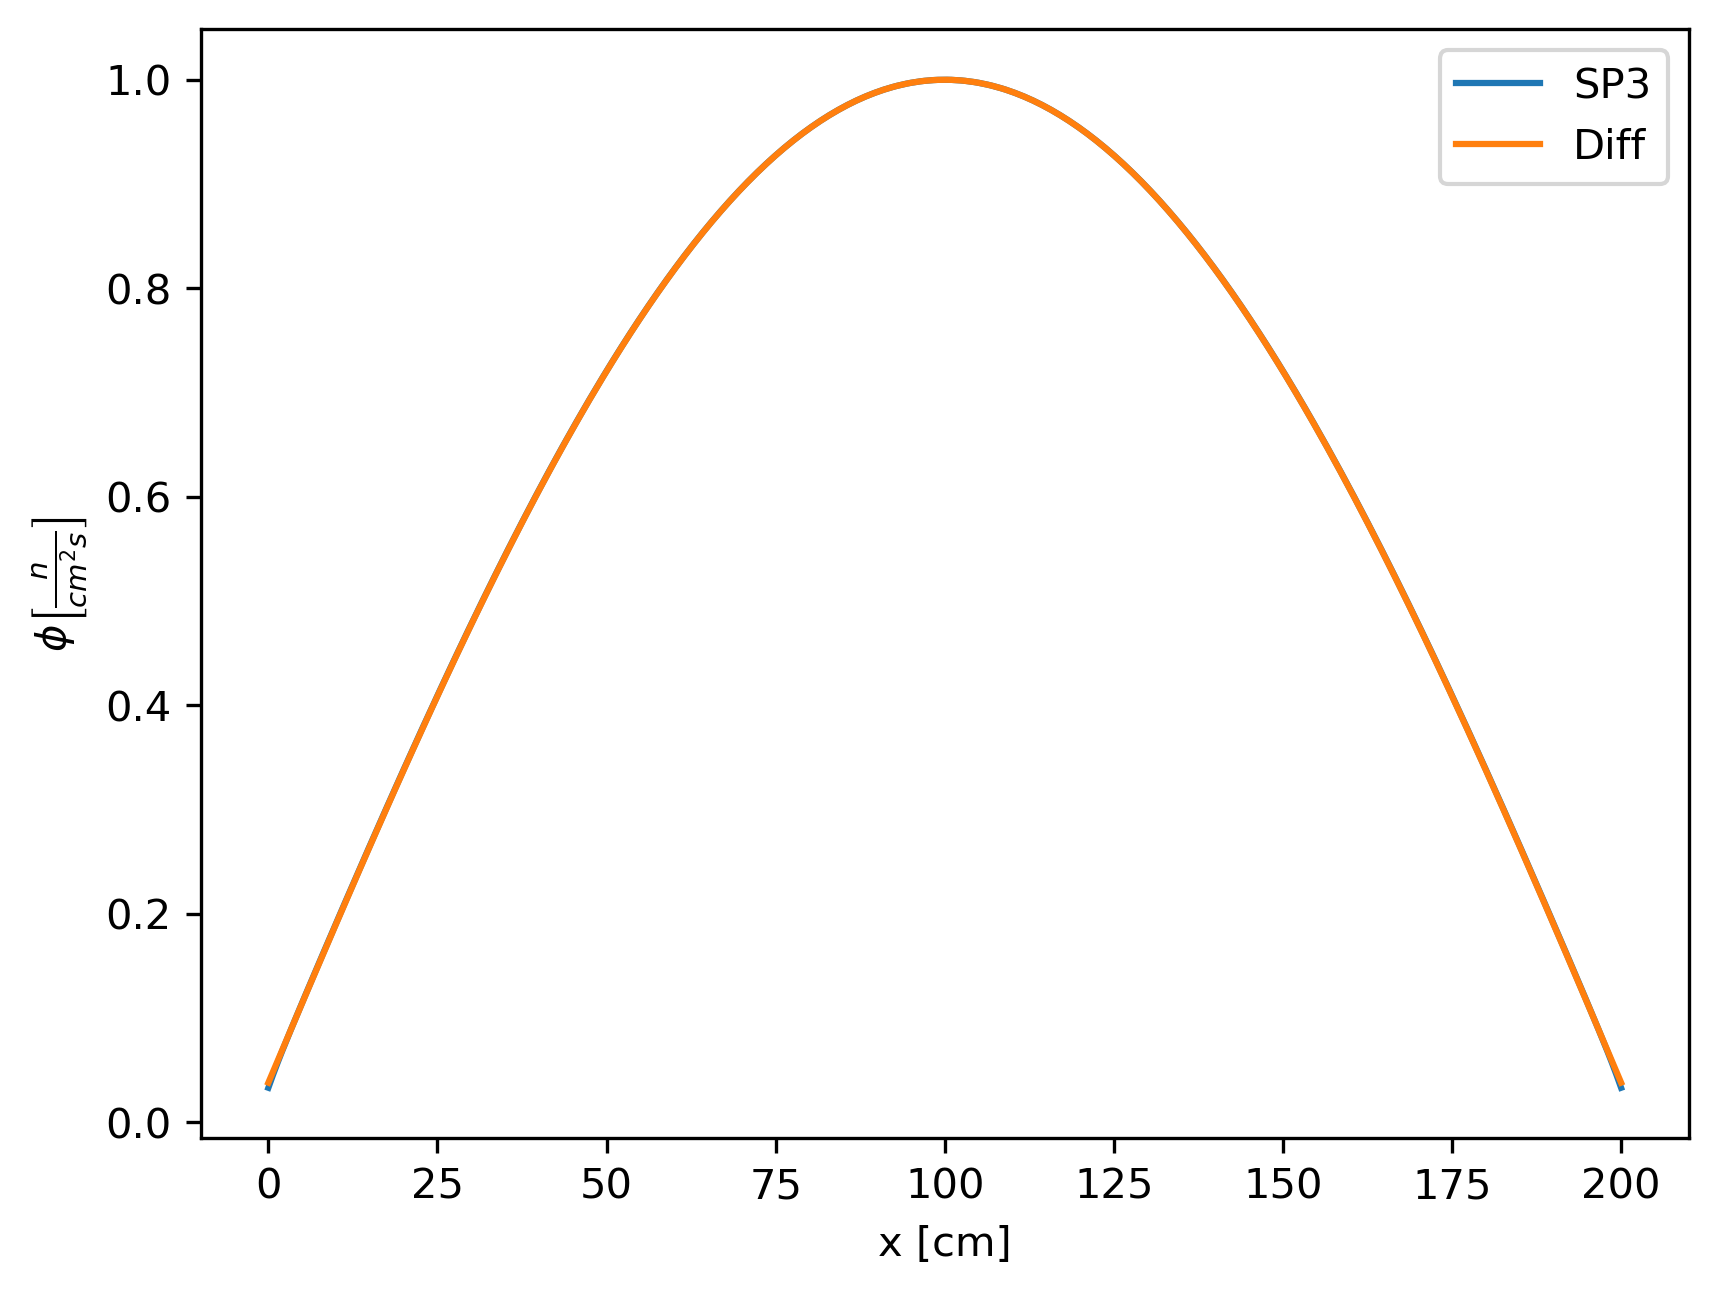
\includegraphics[height=4cm]{../sp3-diffusion/output-1g-crit}
		\end{center}
		\caption{1 group.}
	\end{figure}

	\column[t]{5cm}
	\begin{figure}[htbp!]
		\begin{center}
			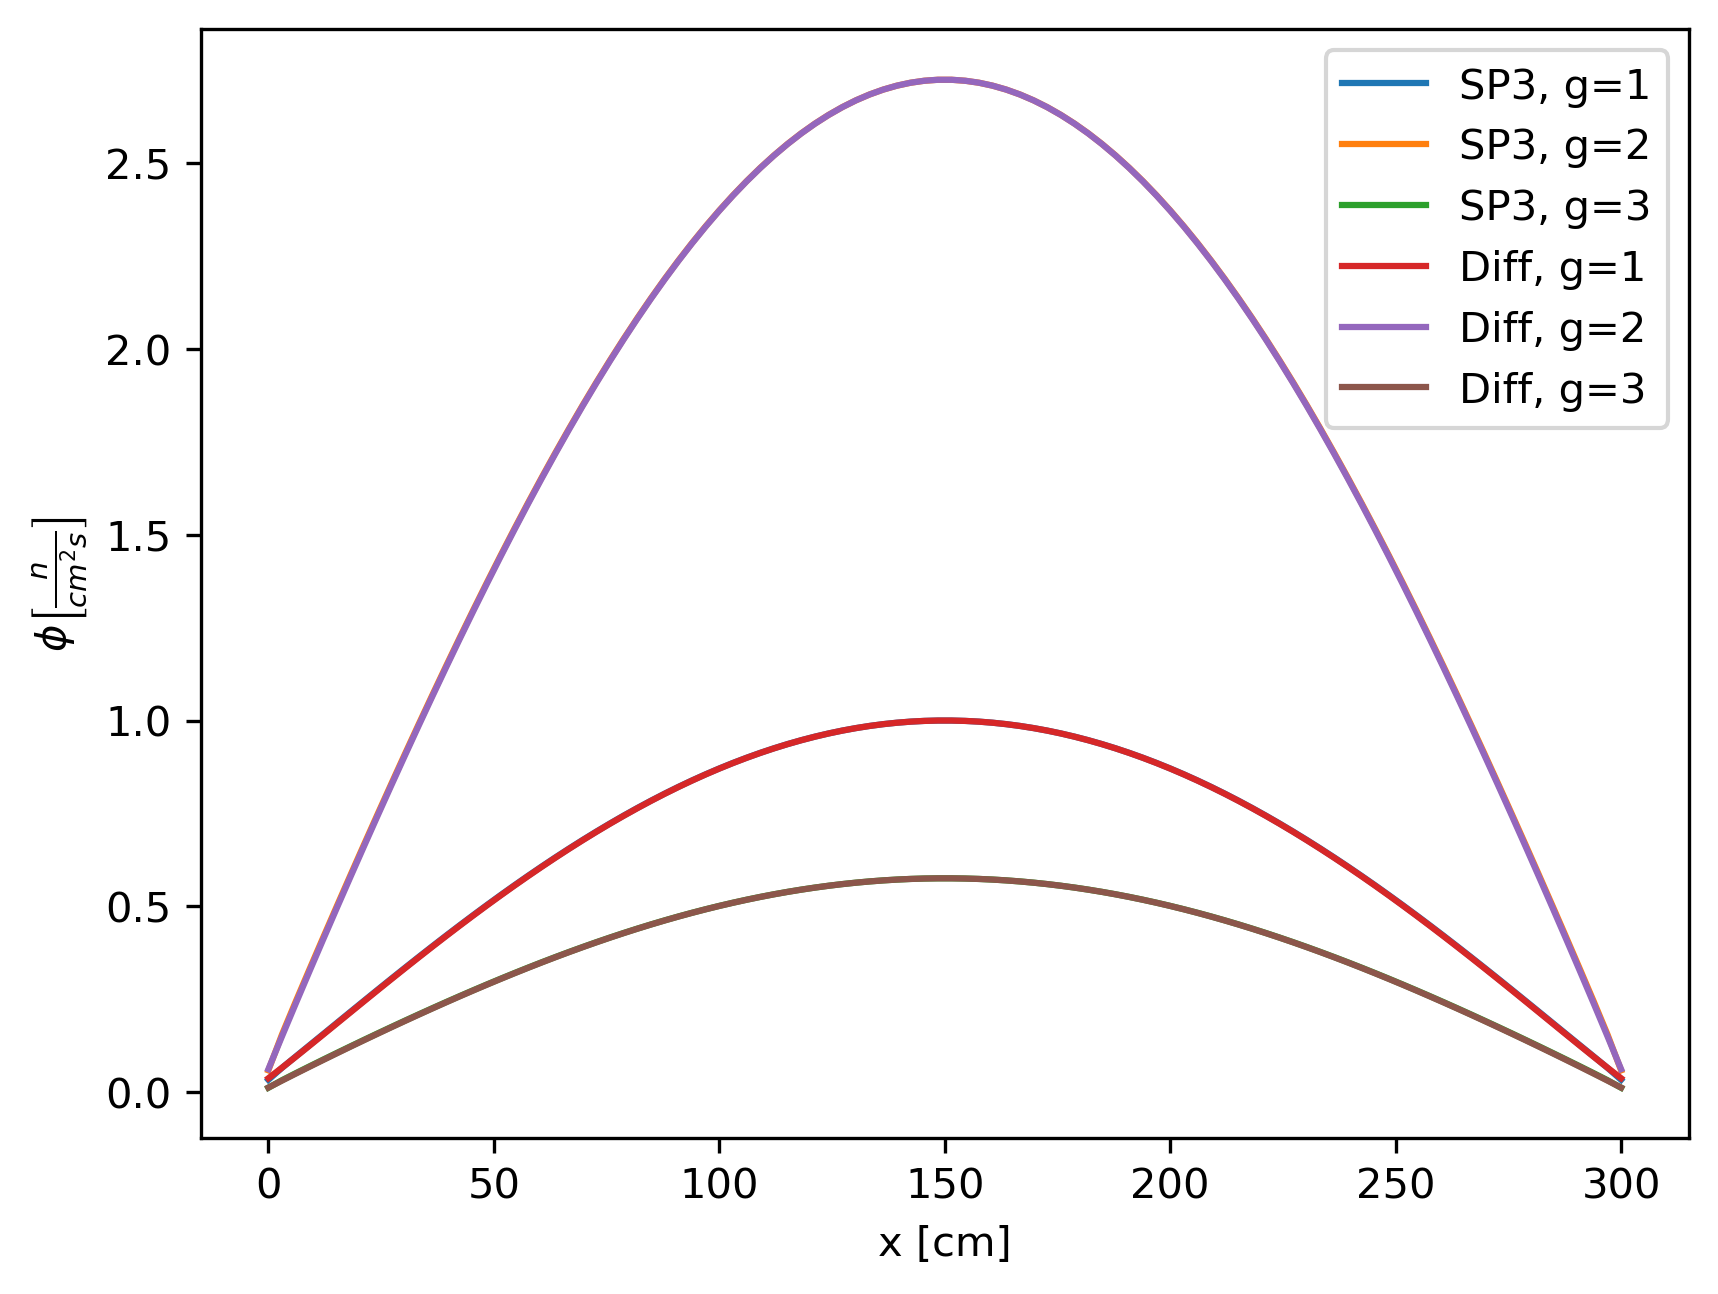
\includegraphics[height=4cm]{../sp3-diffusion/output-3g-crit}
		\end{center}
		\caption{3 groups.}
	\end{figure}
\end{columns}
\end{frame}


\subsection{2-D test case}
\begin{frame}
\frametitle{C5G2 MOX Benchmark}
	\begin{table}[htbp!]
	\centering
	\begin{tabular}{lccc}
	\toprule
	 & C5G2 Benchmark      & \multicolumn{2}{c}{SP3}          \\
	\midrule
	Case & $k_{Ref}$       & $k_{SP_3}$ & $\Delta_\rho$ [pcm] \\
	\midrule
	Heterogeneous & 0.96969  & 0.97106  & 145  \\
	Homogeneous   & 0.96983  & 0.97061  &  83  \\
	\bottomrule
	\end{tabular}
	\label{tab:2d-keff}
	\end{table}
\end{frame}

\begin{frame}
\frametitle{C5G2 MOX Benchmark (2)}
	\begin{figure}[htbp!]
		\begin{center}
			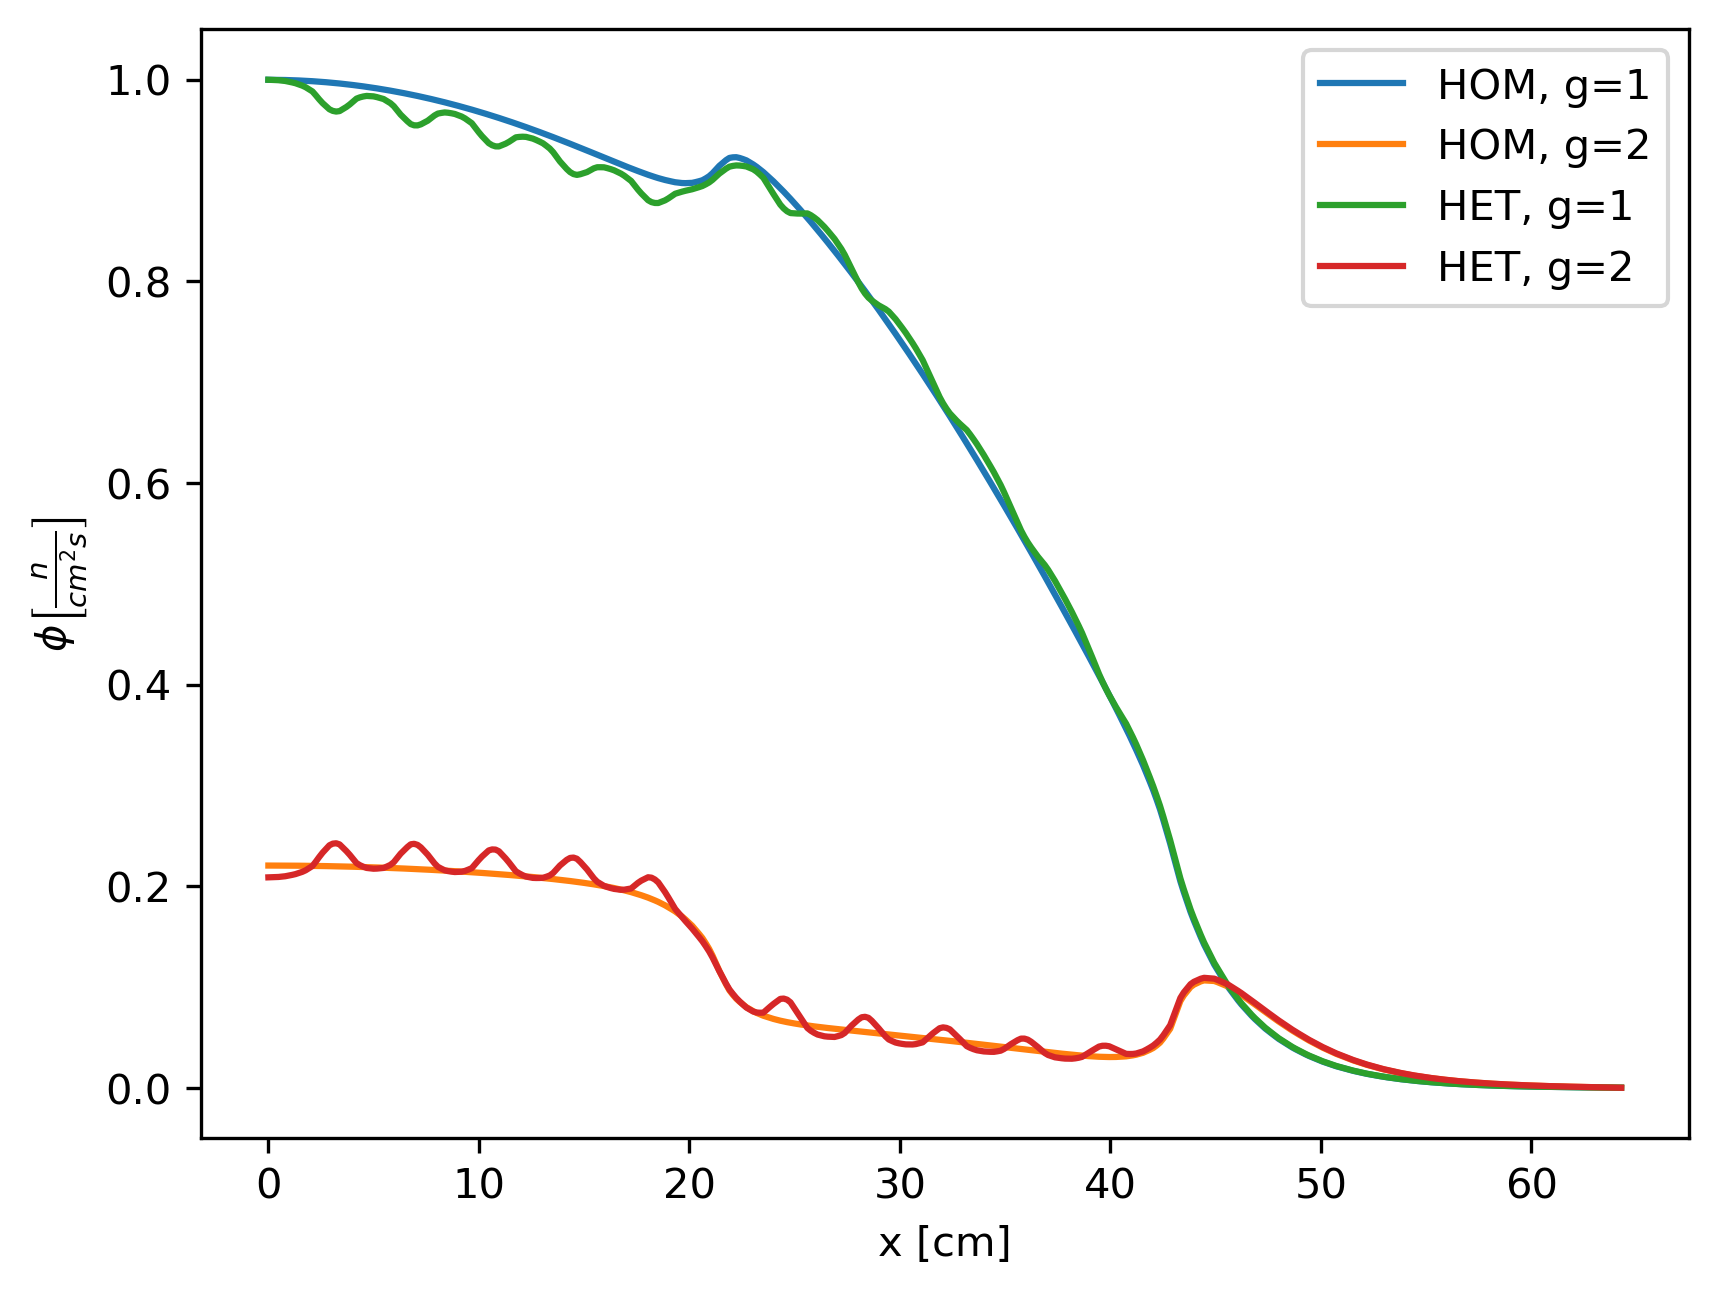
\includegraphics[height=5cm]{{../C5G2-benchmark/output-2g}}
		\end{center}
		\caption{Comparison of the heterogenous and homogeneous cases scalar flux.}
	\end{figure}
\end{frame}

\begin{frame}
\begin{columns}
\frametitle{C5G2 MOX Benchmark (3)}

    \column[t]{5cm}
	\begin{figure}[htbp!]
		\begin{center}
			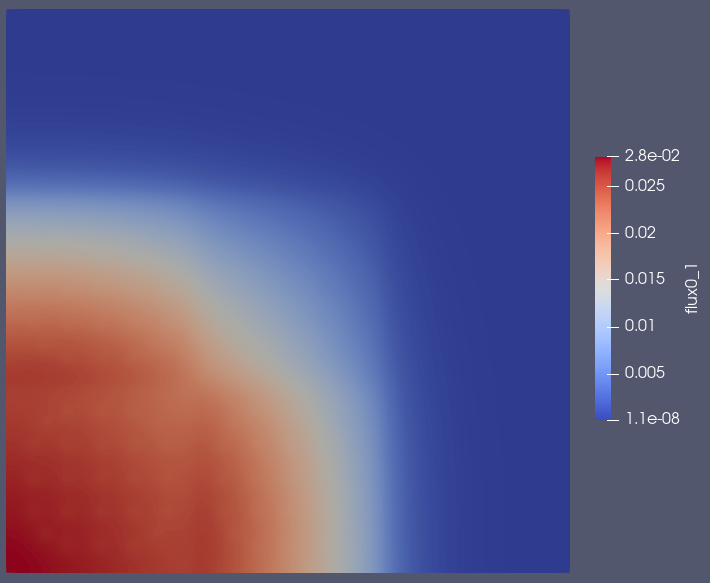
\includegraphics[height=4cm]{flux0_1}
		\end{center}
		\caption{$\Phi_{0, 1}$.}
	\end{figure}

	\column[t]{5cm}
	\begin{figure}[htbp!]
		\begin{center}
			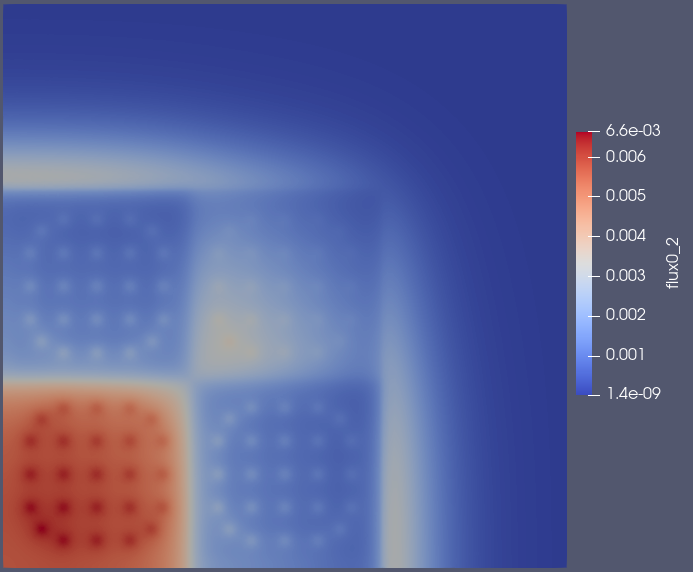
\includegraphics[height=4cm]{flux0_2}
		\end{center}
		\caption{$\Phi_{0, 2}$.}
	\end{figure}
\end{columns}
\end{frame}

\begin{frame}
\frametitle{C5G2 MOX Benchmark (4)}
\begin{columns}
    \column[t]{5cm}
	\begin{figure}[htbp!]
		\begin{center}
			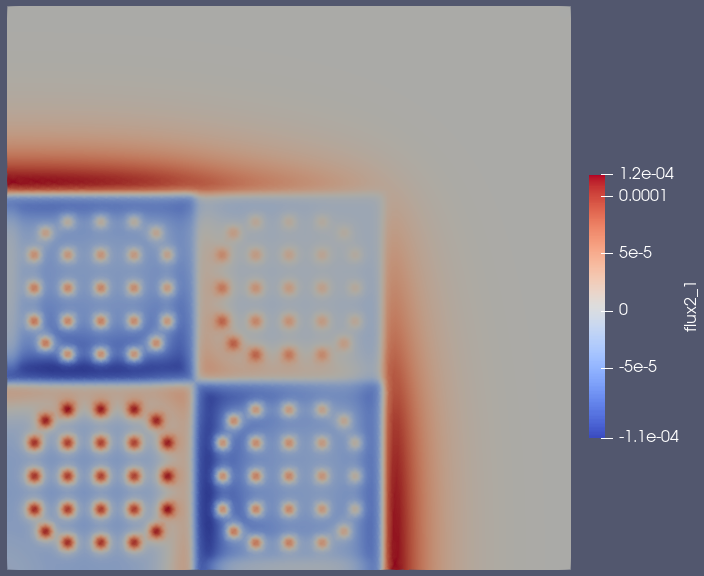
\includegraphics[height=4cm]{flux2_1}
		\end{center}
		\caption{$\Phi_{2, 1}$.}
	\end{figure}

	\column[t]{5cm}
	\begin{figure}[htbp!]
		\begin{center}
			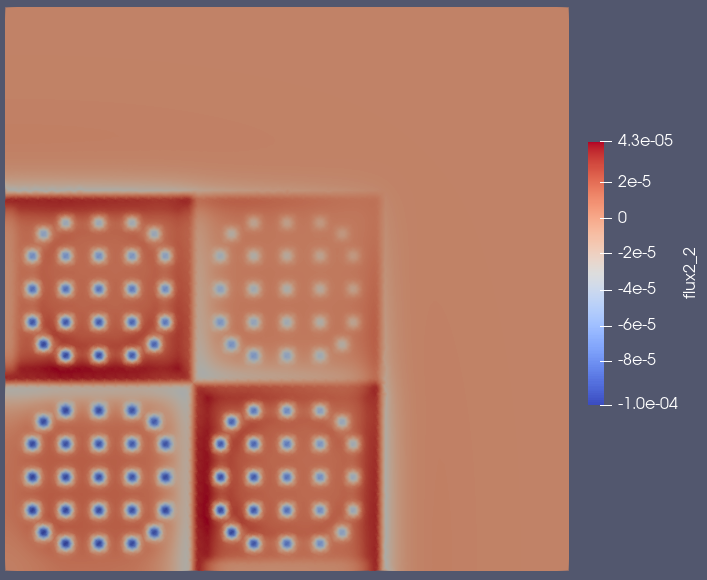
\includegraphics[height=4cm]{flux2_2}
		\end{center}
		\caption{$\Phi_{2, 2}$.}
	\end{figure}
\end{columns}
\end{frame}